\documentclass{report}
\usepackage{fancyhdr} % Required for custom headers
\usepackage{lastpage} % Required to determine the last page for the footer
\usepackage{extramarks} % Required for headers and footers
\usepackage{graphicx} % Required to insert images
%\usepackage{lipsum} % Used for inserting dummy 'Lorem ipsum' text into the template
\usepackage{amsmath}
\usepackage{float}
\usepackage{graphicx} 
%\usepackage{amsfont}
%\usepackage{amssymb}

\usepackage{multicol}
% Margins
\topmargin=-0.5in
\evensidemargin=0in
\oddsidemargin=-0.5in
\textwidth=7.5in
\textheight=9.0in
\headsep=0.25in 


\pagestyle{fancy}

%\rhead{\textbf{Marshall's Recipes}} % Top right header
%\lhead{\textbf{Curry Stir Fry}}
%\chead{ }
%\title{Curry Stir Fry}

\begin{document}
%\vspace{8mm}
%\textbf{PRELIMINARIES:}


\bigskip

\bigskip

\begin{multicols}{2}
\textbf{Ingredients} 
\begin{itemize}
\item 2 cups flour \quad (912 kCal / 28 gP / 2 gF / 196 gC)
\item 3 eggs (room temperature)  \newline (234 kCal / 18 gP / 15 gF / 3 gC)
\item $1\frac{1}{4}$ cup white sugar (968 kCal / 0 gP / 0 gF / 250 gC)
\item 1 stick unsalted butter (softened) \newline (816 kCal / 0 gP / 96 gF / 0 gC)
\item $\frac{1}{2}$ cup milk (room temperature) \newline (75 kCal / 4 gP / 4 gF / 6 gC)
\item $\frac{1}{2}$ cup lemon juice \quad (26 kCal / 0 gP / 0 gF / 8 gC)
\item 1 teaspoon baking powder
\item 1 tablespoon lemon zest
\item $\frac{1}{2}$ teaspoon baking soda 
\item $\frac{1}{4}$ teaspoon salt




\end{itemize}


\columnbreak
\textbf{Procedure:}
\medskip


\begin{enumerate}
\item Preheat the oven to 350 degrees. 


\medskip
\item Grease and flour (or use non-stick spray) a 9 x 5 inch loaf pan.
\medskip

\item Sift together flour, baking powder, soda, and salt. Stir in lemon zest. Set aside.


\item In a large mixing bowl or stand mixer beat butter on medium speed for 2-3 minutes.
\medskip 
\item Gradually add the sugar and continue beating for another 2-3 minutes.
\medskip 
\item Add eggs, one at a time. Make sure you scrape the bottom of your bowl.
\medskip
\item Add lemon juice (the batter will curdle).
\medskip
\item Alternate addition of flour and milk (in 2 additions). Mix on low speed until combined. Do not over mix.
\medskip
\item Bake in preheated oven for 60-75 minutes until golden and cake tester comes out clean.
\medskip
\item Transfer pan to a rack where it can cool down for about 10 minutes before removing loaf to cool down completely on a wire rack.
\medskip \item \textbf{To make icing:} whisk about a quarter cup of lemon juice adding powdered sugar until mixture thickens to a honey-like consistency. Drizzle over a slice for maximum lemon flavor! 
\end{enumerate}
\begin{table}[H]
  \begin{center}
    \caption{Macro totals (just the loaf)}
    \label{tab:table1}
    \begin{tabular}{c|c|c|c} % <-- Alignments: 1st column left, 2nd middle and 3rd right, with vertical lines in between
      \textbf{Calories} & \textbf{Protein} & \textbf{Fat} & \textbf{Carbs}\\
      \hline
      3,031 kCal & 50 g & 117 g & 463 g\\
    \end{tabular}
  \end{center}
\end{table}
\end{multicols}



%\begin{center}
%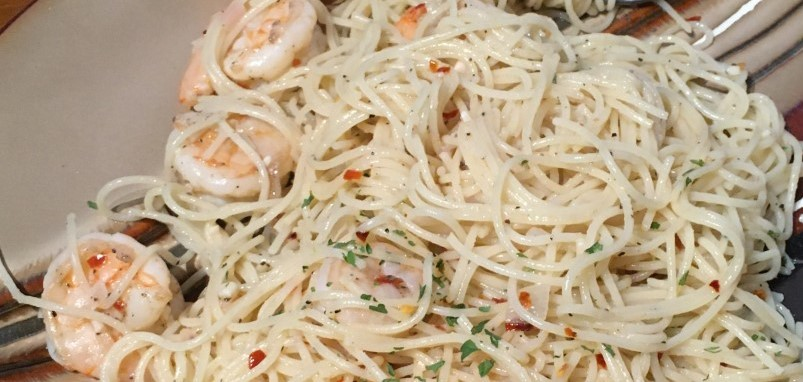
\includegraphics[scale=0.65]{Pasta/Shrimp Scampi/Shrimp Scampi.jpg}
%\end{center}


\end{document}